\documentclass[12pt,a4paper]{article}
\usepackage[utf8]{inputenc}
\usepackage[german]{babel}
\usepackage[T1]{fontenc}
\usepackage{amsmath}
\usepackage{amsfonts}
\usepackage{amssymb}
\usepackage{graphicx}
\usepackage{siunitx}
\usepackage[left=2cm,right=2cm,top=2cm,bottom=2cm]{geometry}
\author{Tim}

\begin{document}
	\setlength{\parindent}{0pt} 
	\begin{center}
		{\LARGE Versuchsprotokoll}\\
		\begin{large}
			zum Grundpraktikum Physik Teil II\\[0.4cm]
			an der RWTH Aachen\\
			I. Physikalisches Institut B\\[4.5cm]
			\Large\textbf{\textsl{E-Lehre}}\\[4cm]
			\normalsize\textit{vorgelegt\\von}\\[0.4cm]
			\large{Moritz Berger\\Tim Herbermann\\Gerald Kolter\\Sebastian Siebert}\\[1cm]
			\large \textit{Gruppe A07} \\ [3cm]
			\large \textbf{Sommersemester 2017}
		\end{large}
	\end{center}
	\newpage
	
	\tableofcontents
	\newpage


\section{Grundlagen}

\subsection{Versuchsbeschreibung}
In den folgenden Versuchen wurde die Güte von Serien- und Parallelschwingkreisen auf verschiedene Arten bestimmt. Zusätzlich wurde in einem letzten Aufbau ein Hoch- bzw. Tiefpass untersucht.

\subsection{Physikalische Grundlagen}

\paragraph{Serienkreis}
Aus der Kirchhoffschen Maschenregel ergibt sich eine Differentialgleichung zur Beschreibung der erzwungenen Schwingung.

\begin{equation}
\frac{U}{L} = \frac{d^2 Q}{dt^2}+\frac{R}{L}\frac{dQ}{dt}+\frac{1}{LC} Q
\end{equation}



Dabei ergibt sich der maximale Strom im Kreis bei Resonanz für
\begin{equation}
\omega_0 = \frac{1}{\sqrt{LC}}
\end{equation} 

Die Güte des Schwingkreises ist definiert durch
\begin{equation}
Q_s = \frac{1}{R} \sqrt{\frac{L}{C}}
\end{equation}

und beschreibt unter anderem den Zusammenhang zwischen angelegter Spannung und Spannungsüberhöhung im Resonanzfall:

\begin{equation}
\frac{U_L(\omega_0)}{U(\omega_0)} = Q_s 
\label{equ:Güte_Spannungsüberhöhung}
\end{equation}

Man stellt fest, dass die Güte sich auch noch als Quotient aus Resonanzfrequenz und Breite der Resonanzkurve bestimmen lässt:
\begin{equation}
\dfrac{\omega_0}{\Delta \omega} = \dfrac{\omega_0}{2d} = \dfrac{\omega_0 L}{R} = \dfrac{1}{R \omega_0 L} = \dfrac{1}{R} \cdot \sqrt{\dfrac{L}{C}} =: Q_S
\label{equ:Güte_Resonanzbreite}
\end{equation}


\paragraph{Parallelschwingkreis}
Aus der Knotenregel kann ebenfalls eine Differentialgleichung zur Beschreibung des Parallelschwingkreises hergeleitet werden.

Aus dieser kann ebenfalls die Resonanzfrequenz bestimmt werden.

\begin{equation}
\omega_0 = \sqrt{\frac{1-\frac{C}{L}\cdot R_L^2}{LC}}
\end{equation} 

Für große Widerstände im Kreis ergibt sich für die Güte der Schaltung näherungsweise der Zusammenhang:

\begin{equation}
Q_P = \frac{1}{R_L} \sqrt{\frac{L}{C}}
\label{equ:Güte_Bauteile}
\end{equation}

Im Falle des Parallelschwingkreises kommt es bei Resonanz zu einer Stromüberhöhung. Auch hier ergibt sich der Zusammenhang:

\begin{equation}
\frac{(I_L)_0}{I_0} = Q_p
\end{equation}

\paragraph{Hoch -und Tiefpass}
Ein Hoch- bzw. Tiefpass 1. Ordnung besteht aus einer Serienschaltung von Widerstand und Kondensator. Durch Anlegen einer Wechselspannung werden, abhängig davon wo die Spannung abgegriffen wird, entweder große oder kleine Frequenzen blockiert bzw. durchgelassen.

Der Hochpass ergibt sich durch Spannungsabgriff am Widerstand. Die Übertragsfunktion ergibt sich dabei zu:

\begin{equation}
\frac{U_a}{U_e} = \frac{1}{\sqrt{(\frac{1}{\omega C R})^2+1}}
\end{equation}

Den Tiefpass erhält man dann entsprechend durch Abgriff am Kondensator. Die Übertragsfunktion lautet:

\begin{equation}
\frac{U_a}{U_e} = \frac{1}{\sqrt{1+(\omega C R)^2}}
\end{equation}

\section{Serienschwingkreis}

\subsection{Aufbau und Durchführung}

\begin{figure}
\centering
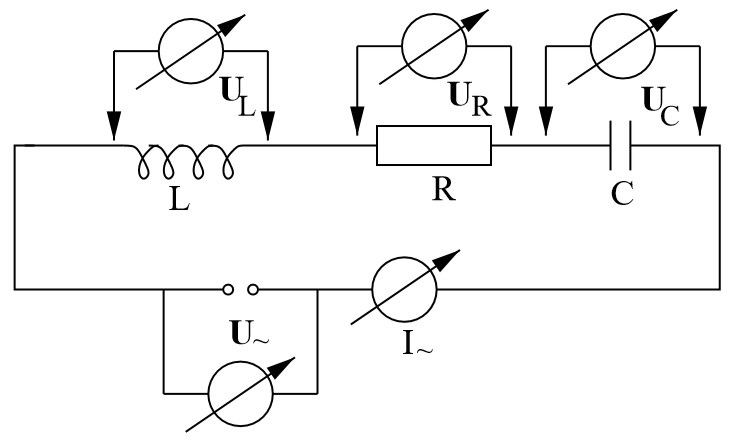
\includegraphics[scale=0.8]{Bilder/AufbauSerie.png}
\caption{Schaltbild zum Serienschwingkreis. Die Spannungsmessung am Ohmschen Widerstand wurde nur im Rahmen der Vorauswertung mit dem Oszilloskop durchgeführt.}
\label{fig:AufbauSerie}
\end{figure}

\subsection{Vorauswertung: Oszilloskop}
Im Rahmen der Vorauswertung wurde die Spannung am Ohmschen Widerstand und die gesamte abfallende Spannung mittels Oszilloskop gemessen. Für Gruppe B wurde der Widerstand mit Nominalwert $R = 5,1 \Omega$ verwendet. Die Frequenz der angelegten Wechselspannung wird über den Frequenzgenerator eingestellt.\\

Zur Bestimmung der Resonanzfrequenz werden die gemessenen Spannungen an beiden Kanälen im Oszilloskop gegeneinander aufgetragen. Die Frequenz wurde so eingestellt, dass die Ellipse verschwindet und die Spannungswerte eine Gerade bilden. Der entsprechende Frequenzwert ist die Resonanzfrequenz
Zur Bestimmung der Resonanzbreite werden in der Zeitdarstellung des Oszilloskops diejenigen Frequenzen bestimmt, für die die Amplitude der Spannung am Widerstand um den Faktor $\sqrt{2}$ kleiner als im Resonanzfall ist. 

Es gilt

\begin{equation}
\Delta f = f_2 - f_1 \quad \Rightarrow \quad Q = \frac{f_0}{\Delta f}
\end{equation}

und mittels Fehlerfortpflanzung:

\begin{equation}
\sigma_{\Delta f} = \sqrt{\sigma_{f_1}^2+\sigma_{f_2}^2} \qquad \sigma_Q = Q \sqrt{(\frac{\sigma_{f_0}}{f_0})^2 + (\frac{\sigma_{\Delta f}}{\Delta f})^2}
\end{equation}

Die Ergebnisse der Voruntersuchung sind für beide Gruppen in Tabelle \ref{tab:Voruntersuchung} dargestellt.

\begin{table}
\centering
\begin{tabular}{|c|c|c|c|c|}
\hline
Gruppe & $f$/Hz & $f_1$/Hz & $f_2$/Hz & Q\\
\hline
A & & & &\\
\hline
B & $2149 \pm 2$ & $1755 \pm 4$ & $2614 \pm 4$ & $2,50 \pm 0,02$\\
\hline
\end{tabular}
\caption{Ergebnisse der Voruntersuchung mittels Oszilloskop}
\label{tab:Voruntersuchung}
\end{table}


Eine zweite Voruntersuchung durch Bestimmen der Spannungsüberhöhung im Resonanzfall war aus Zeitgründen nicht möglich.

\subsection{Auswertung}
Zur Bestimmung der Güte eines Serienschwingkreises gibt es die folgenden 4 Möglichkeiten:
\begin{enumerate}
\item Man misst die Resonanzfrequenz und die Breite der Resonanzkurve. Die Güte ist dann gemäß Gl. \ref{equ:Güte_Resonanzbreite} der Quotient aus beiden.
\item Ein analoges Verfahren lässt sich mit der Phasenverschiebung durchführen: Die Resonanzfrequenz ist dann bei $\varphi = 0$ und die Breite $\Delta \omega$ ist zwischen $\varphi = \pm \ang{45}$.
\item Gemäß Gl. \ref{equ:Güte_Spannungsüberhöhung} lässt sich die Güte auch aus der Spannungsüberhöhung an der Resonanzfrequenz bestimmen.
\item Mit Gl. \ref{equ:Güte_Bauteile} kann die Güte aus den Größen der Bauteilen berechnet werden.
\end{enumerate}
\subsubsection{Gruppe A}




\section{Parallelschwingkreis}

\section{Hoch- und Tiefpass}





\end{document}